
\subsection{Time references, intervals and CPG sequence}
\label{subsec:intervals}
The variability study addressed in this chapter is based on the characterization of cycle-by-cycle intervals in the rhythm produced by the model CPG.
In our analysis of variability, we assess the presence of linear relationships between the intervals that build the sequence and the cycle-by-cycle period to characterize and unveil similar dynamical invariants as those found in the stomatogastric CPG \cite{elices_robust_2019}. 
The intervals here analyzed can be measured for any three neurons following a robust triphasic rhythm. In this paper N1, N2 and N3 represent the feeding CPG phases, represented in the model by interneurons N1M, N2v and N3t, respectively and in the experimental data by different combinations of moto- and interneurons.

\begin{figure}[hbt!]
	\centering
	\begin{minipage}{\textwidth}
		\centering
		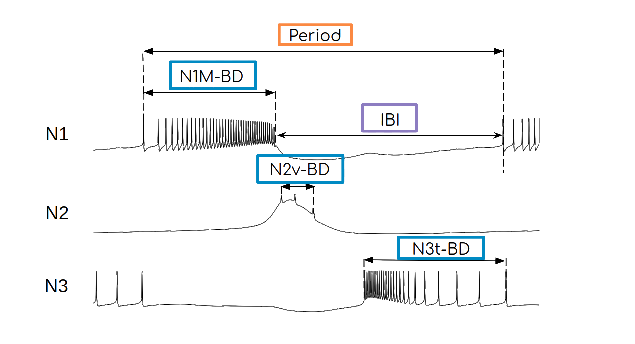
\includegraphics[width=0.8\textwidth]{img/methods-paper-modelo/figure4a.eps} 
		\label{fig:intervals_bd}
	\end{minipage}
	% \hfill
	
	\vspace{1cm}
	\begin{minipage}[t]{\textwidth}
		\centering
		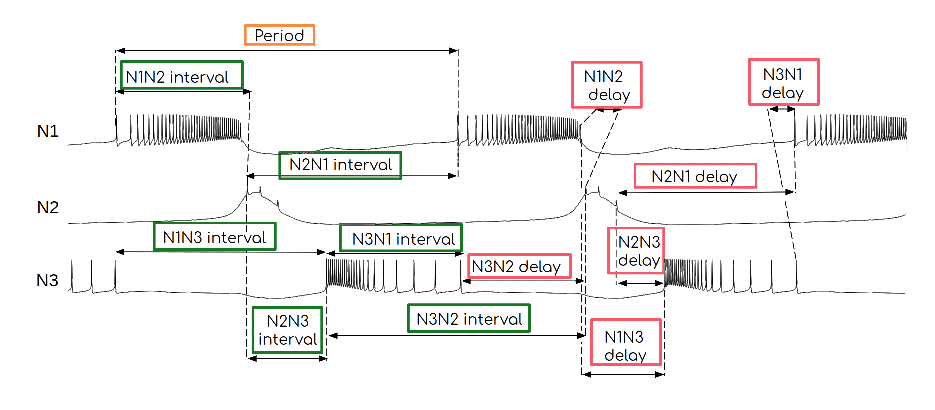
\includegraphics[width=\textwidth]{img/methods-paper-modelo/figure4b.eps} 
		\label{fig:intervals_der}
	\end{minipage}
	
	\caption{\textbf{Panel A}. Individual neuron sequence interval definitions. Each BD label represents the burst duration, defined as the time interval from the first spike to the last spike in the neuron's burst. Period was measured as the interval from the first spike of N1 burst to the first spike of the next N1 burst, covering three phases %(N1M,N2v, N3t) 
		in relation to the activity of the other neurons. IBI represents the interburst interval, defined as the time from the last spike of a neuron's burst to the first one of the next burst in the same neuron.
		\textbf{Panel B}. Definition of intervals involving pairs of neurons. NXNY interval represents interval from NX start to NY start. NXNY delay represents interval from NX end to NY start. Period was measured from N1 start to N1 start, covering the three phases of the CPG rhythm.
	}
	
	\label{fig:intervals}
\end{figure}


This is illustrated in Fig. \ref{fig:intervals}, where single neuron intervals and intervals defined between neurons are depicted and the definition of each interval is as follows:
\begin{enumerate}
	\item \textbf{Burst Duration (BD)}, measured as the time interval between the first and the last spike of the burst (start to end in the trace of a given neuron).
	\item \textbf{Inter Burst Interval (IBI)}, characterized as the difference between the last spike of a burst and the first one of the next one (end to start in the trace of a given neuron).
	\item \textbf{Period}, which envelops the bursts from the three neurons, measured as the distance between the first spike of one burst in a neuron and the first spike of the next one on that neuron (start to start).
	\item \textbf{NeuronX-NeuronY interval}, this interval is measured from the start of the burst of neuron X to the start of the burst of neuron Y (start X to start Y).
	\item \textbf{NeuronX-NeuronY delay}, being the time lapse between the burst end of a neuron X and the burst beginning of neuron Y. (end X to start Y).
\end{enumerate}

Note that it is also possible to define those intervals only with the references from two neurons. For example, the intervals conformed based on N1 and N3 intervals would be: N1N3 and N3N1 intervals and N1N3 and N3N1 delay. Note that the intervals corresponding to the third neuron are enclosed in the others defined, e.g., in this example N2 burst and N2N1 delay would be contained in N1N3 delay. This consideration allows the characterization of the variability cycle-by-cycle in cases where it is not possible to define time references for the three neurons in the circuit. 

\subsection{Inducing variability in the model by current injection}
\label{subsec:inj protocol}
The spiking-bursting activity of the model CPG neurons can be modulated by using an additional current injection on each cell, implemented in the \(i_{inj}\) term of equation (\ref{eq:soma}), as performed in many experimental protocols. Depending on the current value applied, the corresponding neuron dynamics changes. While for N2v a change in this injection corresponds to a change in burst frequency (i.e. the number of bursts increases/decreases), for the rest of the neurons in the model a change in \(i_{inj}\) affects burst duration for N3t and SO, and the length of the depolarization phase in N1M.


\begin{figure}[hbt!]
	\centering
	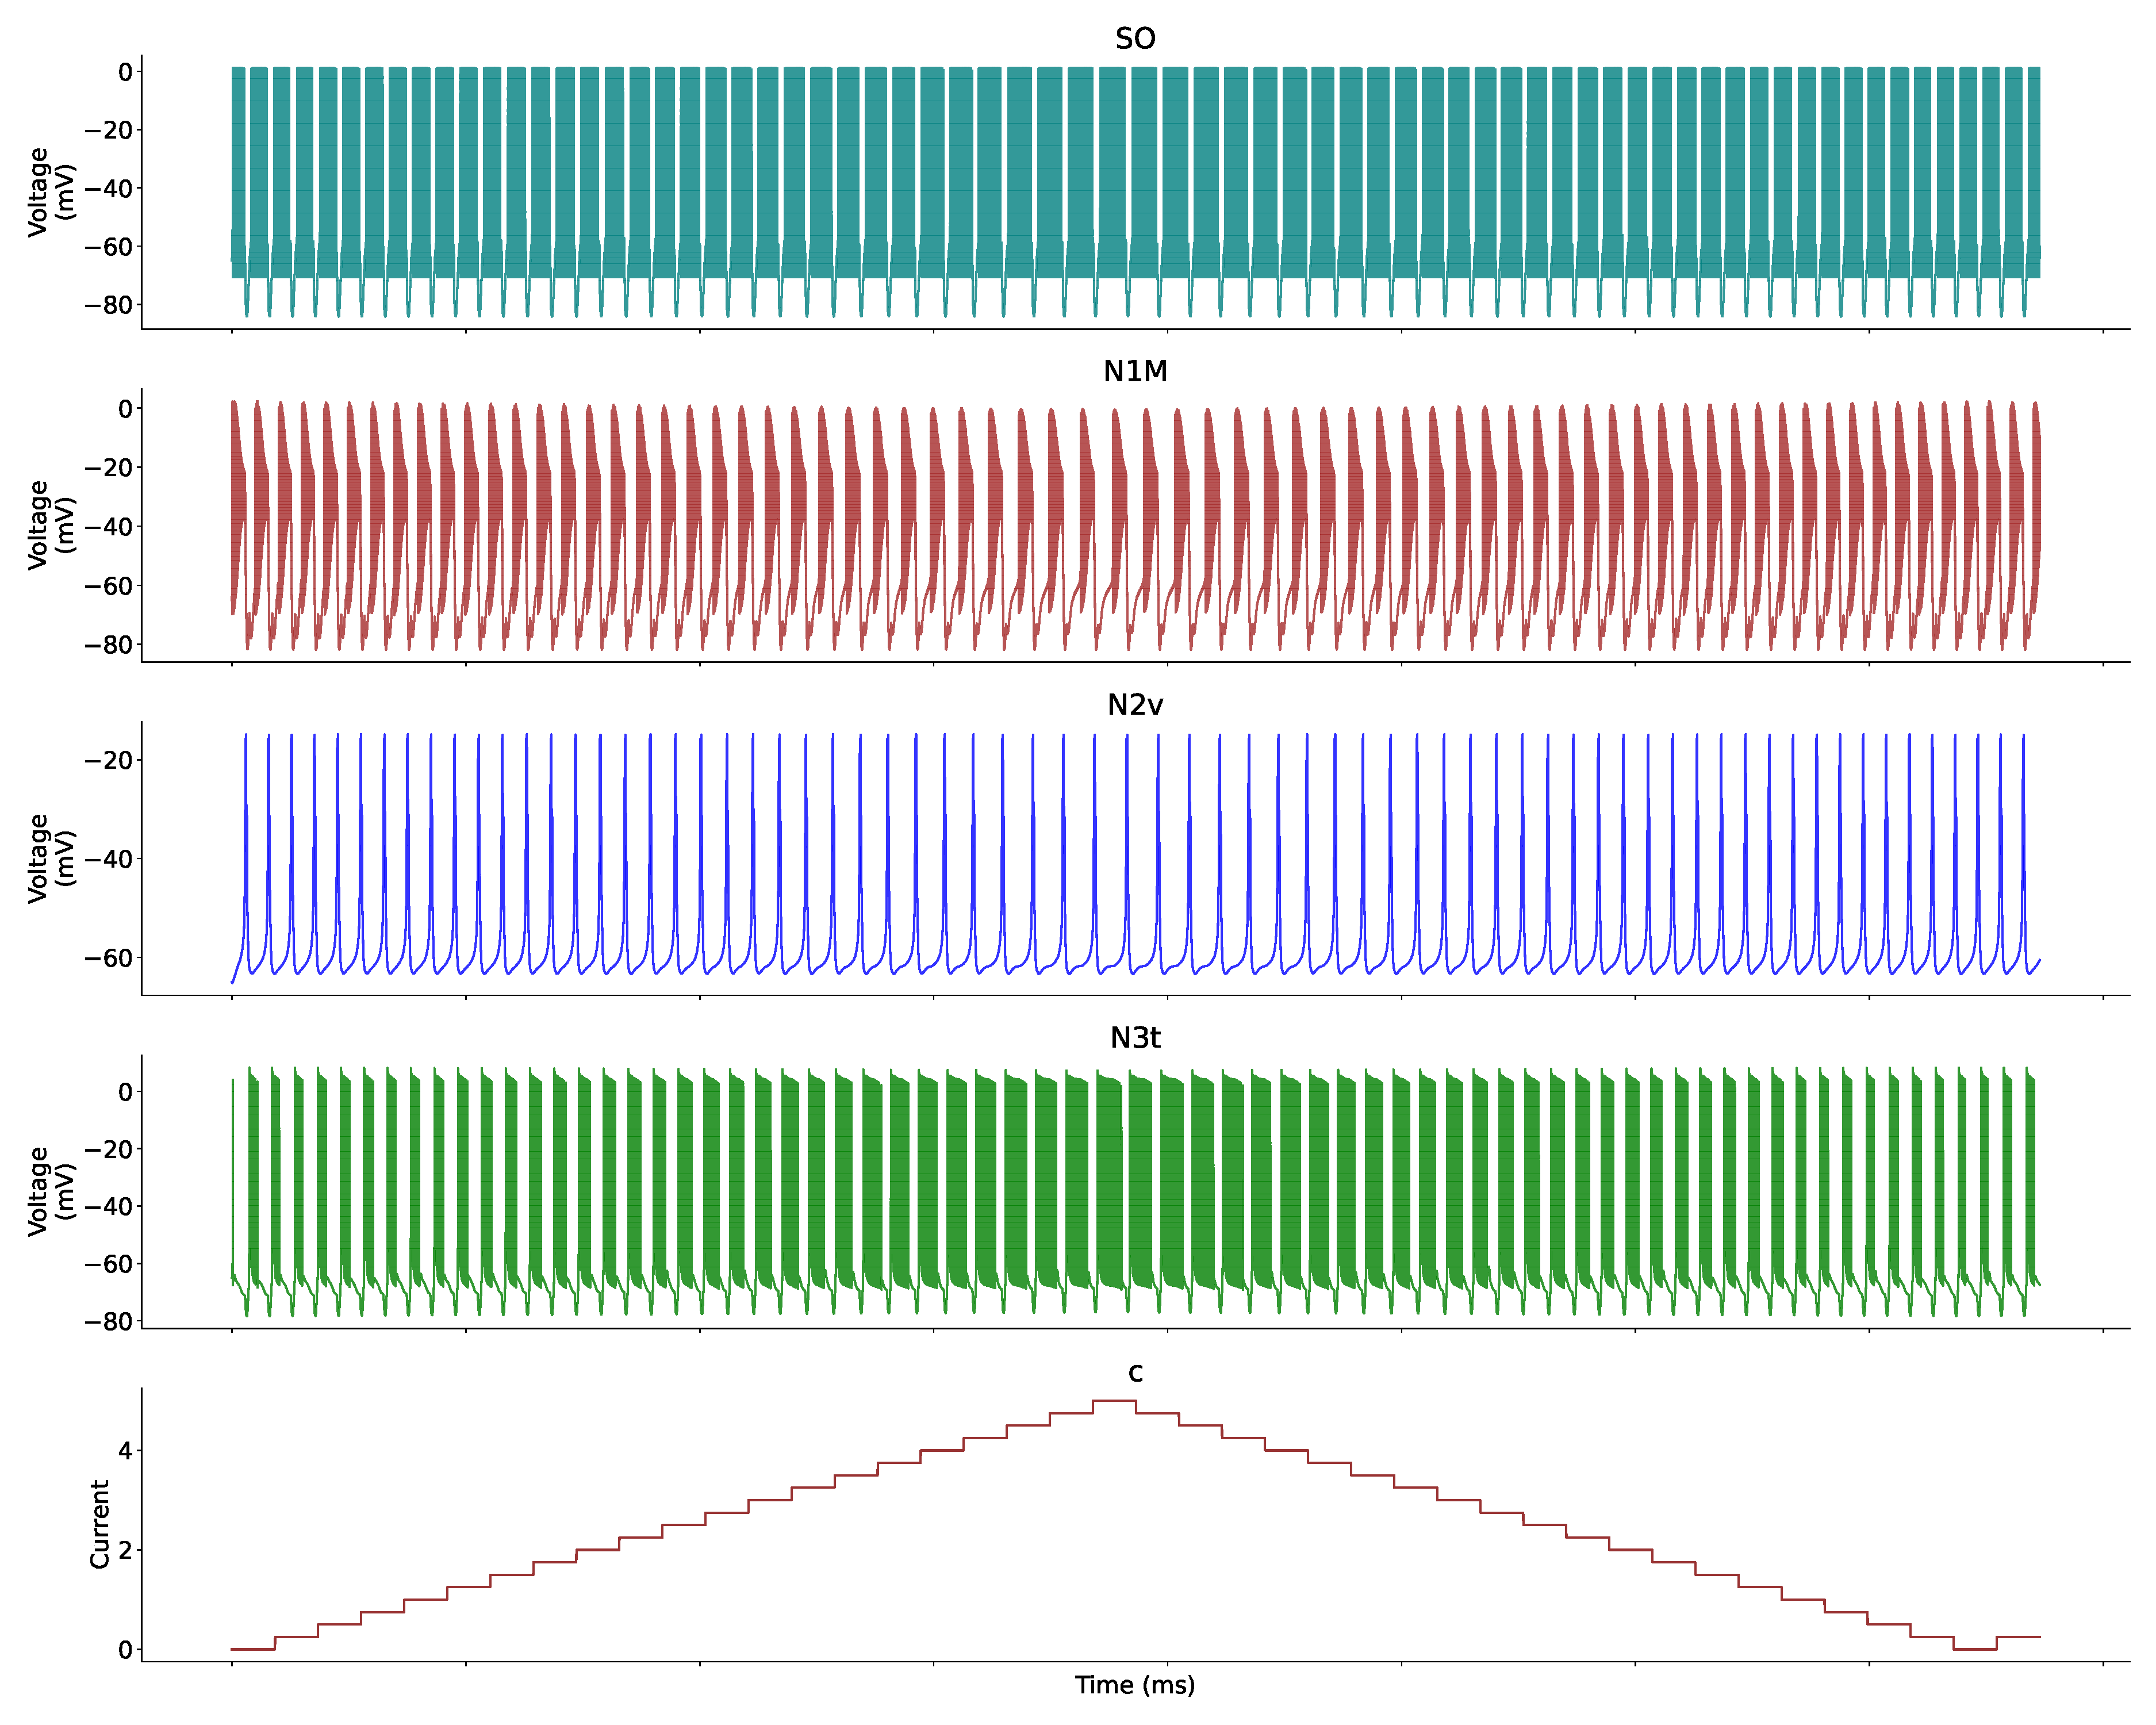
\includegraphics[width=\textwidth]{img/methods-paper-modelo/circuit_w_current.pdf}
	\caption{Illustration of the CPG activity when a current ramp \(i_{inj}\) is applied to N3t. Variability in the sequence intervals was induced by applying two consecutive ramps as the one shown in this figure into different cells.  }
	\label{fig:complete ramp example}
\end{figure}

Whilst the single neuron model descriptions have no intrinsic variability, the effect produced by the modulation of the injected current in each neuron induces variability into the circuit, which allows characterizing the sequence intervals and the period, the associated robustness of the rhythm and the presence of dynamical invariants. Such stimulation has been used previously in the living circuit, as reported by \cite{Elliott1991}. The authors of this work showed that it is possible to activate the feeding CPG with variability caused by current injection into individual cells in the circuit. CPG rhythms obtained under this type of stimulation differ depending on which neuron is being stimulated. To induce variability in the model we used a ramp protocol resulting in circuit time-interval variations as in Fig. \ref{fig:complete ramp example}.

% Even though this CPG model do not present intrinsic variability, thanks to the current \(i_{inj}\), variability is induced into the model, effectively changing burst duration. This current injection has also been used in Lymnaea preparation in living elements, stimulating N1M and SO, obtaining rhythm. Neural sequences obtained after the stimulation differ one another depending on which neuron is being stimulated. 


By varying the current injected into N1M, its burst duration is kept nearly constant, but its depolarization phase before the spiking activity begins becomes longer. Since N3t is the neuron fitting in the sequence in that phase (see Fig. \ref{fig:model simulation}), it also increases its burst duration, being the most variable one in the CPG rhythm. 

When value \(i_{inj}\) is increased on neuron SO, its burst duration becomes longer. Since SO has a modulator effect over N3t and N1M, it also alters the burst duration of these two neurons.

Neuron N3t also shows variable burst duration when an evolving current is injected. When \(i_{inj}\) value on N3t is larger, its burst duration increases, elongating the N1M depolarization phase.  

Finally, when current is applied to N2v the effect on its burst duration or the burst duration of the rest of the neurons is rather small. However, \(i_{inj}\) % current 
modulates N2v burst frequency through the hyperpolarization phase. 

%cambios
Therefore, we used a current ramp protocol to induce variability in the CPG model defined as follows: a ramp variable $c$, which controlled the current injection value ($i_{inj}=c$) on the neuron being stimulated, was increased from a minimum to a maximum value, and then decreased back to the initial value. This was repeated twice in each simulation. The ramp variable was modified with a fixed step value every 4.6 seconds (the approximate duration of two N3t bursts). The minimum and maximum $c$ values were different in each cell and were tuned to generate realistic spiking-bursting behavior. All parameters used for the simulation analyses reported in this paper are summarized in Table \ref{table:inj values}.

\begin{table}[h!]
\centering
\begin{tabular}{c|cccc|c|ccc|}
\multirow{2}{*}{\textbf{\begin{tabular}[c]{@{}c@{}}Neuron\\ stimulated\end{tabular}}} & \multicolumn{4}{c|}{\textbf{\(i_{inj}\) value}}                 & \multirow{6}{*}{} & \multicolumn{3}{c|}{\textbf{Ramp values ($c$)}}   \\ \cline{2-5} \cline{7-9} 
                                                                                      & \textbf{SO} & \textbf{N1M} & \textbf{N2v} & \textbf{N3t} &                   & \textbf{Min} & \textbf{Max} & \textbf{Step} \\ \cline{1-5} \cline{7-9} 
\textbf{N1M}                                                                          & 8.5         & $c$            & 2            & 0            &                   & 0            & 10.5         & 0.5           \\ \cline{1-5} \cline{7-9} 
\textbf{N3t}                                                                          & 9           & 10           & 1            & $c$            &                   & 0            & 5            & 0.25          \\ \cline{1-5} \cline{7-9} 
\textbf{SO}                                                                           & $c$           & 10           & 1            & 4            &                   & 8.2          & 13           & 0.25          \\ \cline{1-5} \cline{7-9} 
\end{tabular}
\caption{List of \(i_{inj}\) values that yield realistic bursting rhythms for each neuron in the model CPG used in the stimulation protocols reported in this paper. The left section of the table displays the \(i_{inj}\) values applied to each neuron (columns) during each simulation condition (rows). Ramp values on the right section refer to the minimum and maximum values of the ramp variable $c$ in each simulation, increasing \(i_{inj}\) in the specified step every 4.6 seconds (the approximate duration of two N3t burst) to induce variability.} \label{table:inj values}
\end{table}

Simulations of \cite{vavoulis_computational_2007} model were implemented in C++. The code of the feeding CPG model implementation is available at \href{github.com/GNB-UAM/CPG-feeding-Lymnaea}{https://github.com/GNB-UAM/CPG-feeding-Lymnaea}. This model was also included in Neun library in a Github repository \href{github.com/GNB-UAM/Neun}{https://github.com/GNB-UAM/Neun}. Each simulation had the duration of two consecutive cycles of up and down ramps as the one shown in Fig. \ref{fig:complete ramp example} using the parameters described in Table \ref{table:inj values}. The number of bursts in each simulation was approximately 140 (this number slightly depends on the neuron stimulated). Parameter values such as reversal potentials and synaptic conductances were the same ones specified in \cite{Vavoulis2007}.


% \subsection{Model simulation specifications and statistical analysis}\todo{añadir en métodos generales o ampliarlo también a experimental}



\subsection{Experimental recordings and stimulation}
The experimental recordings analyzed in section \ref{sec:experimental sussex} were performed by Michael Crossley, University of Sussex, and kindly provided for this work. 

Each recording had at least 5 microelectrodes, which allowed to characterize the rhythm based on combinations of different neuron's activity. There are cases of experiments in that section:
\begin{itemize}
	\item Spontaneous activity: After the isolation of the CNS, the electrodes impailed in the neuron recorded the spontaneous activity in the CPG, with no further stimulation.
	\item Nerve electrical stimulation: For the activation of the rhythm it is possible to stimulate the median lip nerve (MLN). The data analyzed there was stimulated by a 4V stimulous at 1Hz. 
	\item Neuron electrical stimulation: To modulate the CPG rhythm, SO and CV1a neurons where stimulated (in different experiments) by injecting a constant depolarizing current.
\end{itemize}

%To define each phase, we used different neurons and bursting references, depending on the ones available on the circuit, following intervals definition in table \ref{table:cpg ref intervals}.
%
%For each recording each phase was defined as follows:
%
%\paragraph{Spontaneous Activity Example 1}
%N1 phase was analyzed from B1 activity (bursting and depolarization); N2 phase was analyzed from B5 hyperpolarization, which has a strong inhibition from N2v; N3 phase was analyzed from the bursting activity of B8, that replicates the N3t duration. 
%
%\paragraph{Spontaneous Activity Example 2}
%N1 phase was analyzed from B1 activity (bursting and depolarization); N2 phase was analyzed from B1 hyperpolarization, which has a strong inhibition from N2v; N3 phase was analyzed from the bursting activity of B8, that replicates the N3t duration. 
%Since the reference for N2 here coincides with N1 reference, we display here only the intervals corresponding to N1 and N3 phases, since the intervals that correspond to 3 phases, such as N1-N2 delay or N2-N3 delay, either are already represented in the defined intervals or have a duration close to 0 ms.
%
%\paragraph{Spontaneous Activity Example 3}
%N1 phase was analyzed from B1 activity (bursting and depolarization); N2 phase was analyzed from B5 hyperpolarization, which has a strong inhibition from N2v; N3 phase was analyzed from the bursting activity of B8, that replicates the N3t duration. 
%
%\paragraph{Spontaneous Activity SO modulation}
%N1 phase was analyzed from B1 activity (bursting and depolarization); N2 phase was analyzed from B5 hyperpolarization, which has a strong inhibition from N2v; N3 phase was analyzed from the bursting activity of B8, that replicates the N3t duration. 




\subsection{Models with chaotic activity}

\subsubsection{LP model by \cite{nowotny_probing_2008}}

The membrane potential of axon and soma compartment, $V_{\text{axon}}$ and $V_{\text{soma}}$ respectively, are described by

\begin{equation}
	\frac{dV_{\text{axon}}}{dt} = \frac{1}{C_a} \left( -I_{\text{Na}} - I_{\text{Kd}} - I_M - I_{\text{leak,a}} + I_{VV} \right)
\end{equation}

\begin{equation}
	\frac{dV_{\text{soma}}}{dt} = \frac{1}{C_s} \left( -I_{\text{Ca}} - I_{\text{KCa}} - I_A - I_h - I_{\text{leak,s}} - I_{VV} + I_{\text{scale}} (I_{\text{DC}} - I_{\text{offset}} + I_{\text{syn}} \right))
\end{equation}

$I_{\text{offset}} = 2 \, \text{nA}$ stems from the residual coupling at the end of the parameter estimation procedure which introduces a current bias due to differences in baseline voltage of data and model (on top of $V_{\text{shift}}$). $I_{\text{syn}}$ denotes the total incoming synaptic current. All ionic currents except for the ones mentioned explicitly below are given by

\begin{equation}
	I_x = g_x m^p h^q (V - V_x)
\end{equation}

where $g_x$ is the maximal conductance of the current, $V$ is the membrane potential of either the axon compartment ($I_{\text{Na}}$, $I_{\text{Kd}}$, and $I_M$) or the soma compartment (all other currents), and $V_x$ is the reversal potential of the current. The activation and inactivation variables are governed by

%\begin{equation}
%	\frac{dm}{dt} = \alpha_m (1 - m) - \beta_m m
%\end{equation}
%
%\begin{equation}
%	\frac{dh}{dt} = \alpha_h (1 - h) - \beta_h h
%\end{equation}
%
%for $I_{\text{Na}}$ and $I_{\text{Kd}}$, and
%
%\begin{equation}
%	\frac{dm_x}{dt} = \frac{m_{\infty,x}(V) - m_x}{\tau_{m_x}}
%\end{equation}

\subsubsection{Non chaotic model \cite{ghigliazza_minimal_2004}}
\todo{revisar}
The Ghigliazza and Holmes model for motoneurons is described by the following equations:

1. The membrane potential dynamics of a neuron is given by:

\begin{equation}
	C_m \frac{dV}{dt} = -\sum I_x + I_{\text{syn}}
\end{equation}

where \( C_m \) is the membrane capacitance, \( V \) is the membrane potential, \( I_x \) are the various ionic currents, and \( I_{\text{syn}} \) is the synaptic current.

2. The ionic currents \( I_x \) are typically given by:

\begin{equation}
	I_x = g_x m^p h^q (V - V_x)
\end{equation}

where \( g_x \) is the maximal conductance, \( m \) and \( h \) are the activation and inactivation variables, \( p \) and \( q \) are the respective powers, and \( V_x \) is the reversal potential of the current.

3. The gating variables \( m \) and \( h \) are governed by first-order kinetics:

\begin{equation}
	\frac{dm}{dt} = \alpha_m (1 - m) - \beta_m m
\end{equation}

\begin{equation}
	\frac{dh}{dt} = \alpha_h (1 - h) - \beta_h h
\end{equation}

where \( \alpha_m \), \( \beta_m \), \( \alpha_h \), and \( \beta_h \) are voltage-dependent rate constants.

4. For a central pattern generator (CPG), the model includes a set of coupled differential equations to describe the rhythmic activity:

\begin{equation}
	\frac{d\phi_i}{dt} = \omega_i + \sum_j K_{ij} \sin(\phi_j - \phi_i - \psi_{ij})
\end{equation}

where \( \phi_i \) is the phase of the \( i \)-th oscillator, \( \omega_i \) is the intrinsic frequency, \( K_{ij} \) is the coupling strength between oscillators \( i \) and \( j \), and \( \psi_{ij} \) is the phase shift.



\subsection{Hybrot structure}
The experimental paradigm designed in order to test the correct behavior and locomotion of the FLC-Hybrot --FLC stands for Functional Living Circuit-- established a real-time closed-loop interaction between the robot and a living pyloric CPG of \textit{Carcinus maenas} \cite{Elices2019}. During the experiment, the FLC-Hybrot had to walk through a straight and flat lane, with no obstacles, along which there were interspersed sections with lights and shadows. Neural activity was recorded online from the living circuit and used to modulate the robot movement. At the same time, feedback current was injected into the living circuit when the robot's light-sensor detected a shadow.

Top panel of Figure \ref{fig:robot_results_setup} shows an illustration of the experimental setup for the FLC-Hybrot implementation with all its main components. A computer was employed to serve as nexus between both the robot and the biological elements and was in charge of executing a periodic real-time loop (Figure \ref{fig:robot_results_setup}A), inside of which the following tasks were performed:
\begin{enumerate}
	\item First, it read the CPG neurons electrophysiological signals from the DAQ device, that at the same came through the amplifiers (Figure \ref{fig:robot_results_setup}B) after being recorded online from the living preparation (Figure \ref{fig:robot_results_setup}C).
	\item From this acquired data it extracted, online, the duration of the temporal intervals of the cycle-by-cycle CPG activity, which were then sent to the robot's controller via Bluetooth.
	\item In the opposite direction, it received the robot's light-sensor data through the same Bluetooth connection.
	\item If this data indicated that the robot was located under a shadow at that moment, then it sent feedback to the DAQ device in the form of electric current. This current was injected into the neurons, delivered by the amplifier, altering their behavior.
\end{enumerate}

All these operations were repeated while the robot traversed the trial track (Figure \ref{fig:robot_results_setup}D). Robot's locomotion was determined by its legs oscillation, so we utilized video tracking tools to capture their movement during the experiment (Figure \ref{fig:robot_results_setup}E). Two electrodes were used in order to measure the pyloric CPG activity. First, an extracellular electrode picked up all the surrounding neurons' activity. In this signal, the spikes and bursts of the LP neuron were clearly recognizable due to their larger amplitude. One of the PD neurons' membrane potential was recorded using an intracellular electrode. A second intracellular electrode was used to inject the feedback current into a PD neuron to implement the robotic sensory feedback (Figure \ref{fig:robot_results_setup}F).

\begin{figure}[h!]
	\begin{center}
		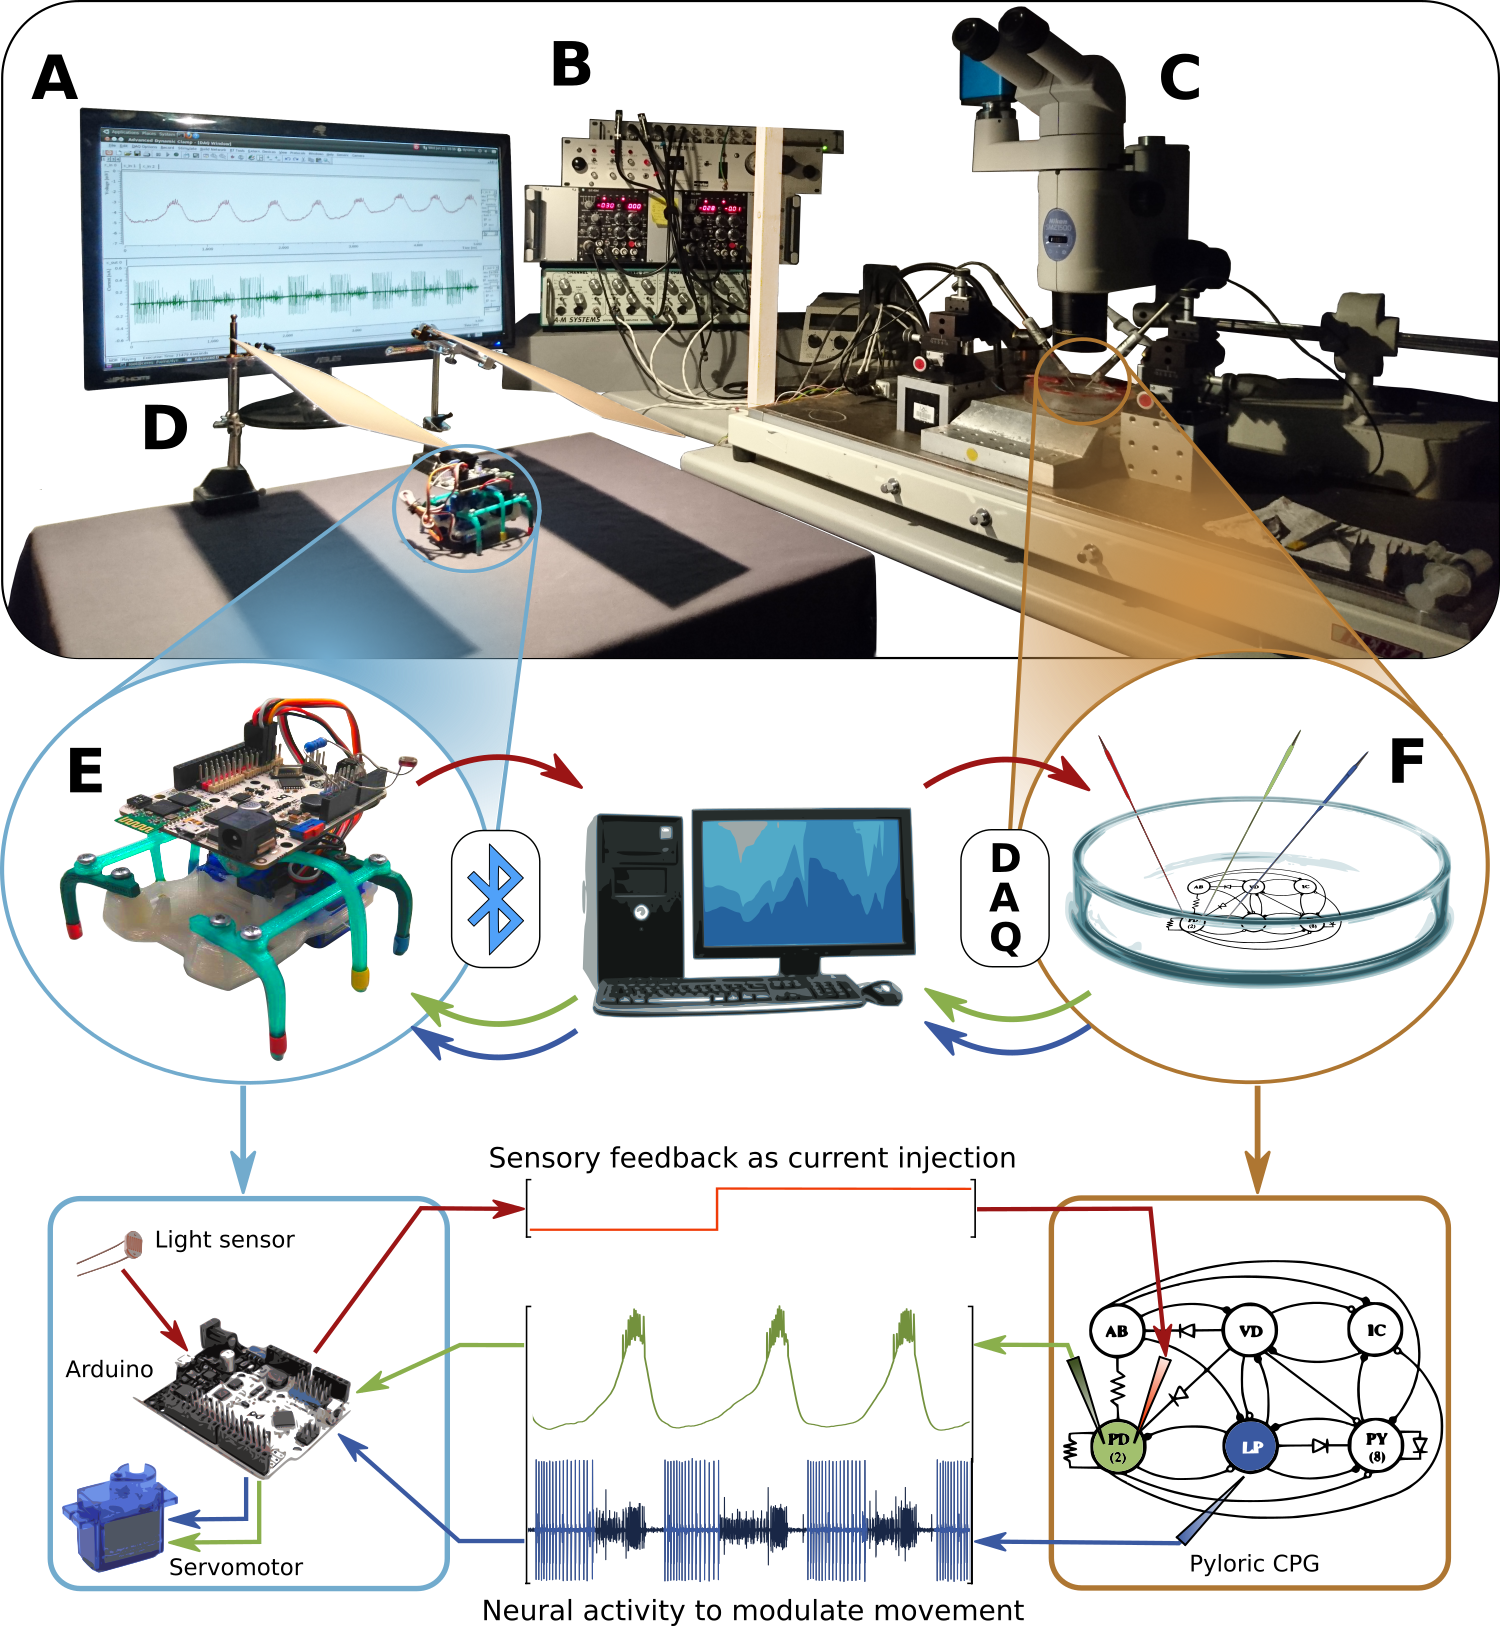
\includegraphics[width=0.65\linewidth]{img/invariants/robot/robot_results_setup.png}
	\end{center}
	\caption{\textbf{Top panel:} illustration of the experimental setup for the FLC-Hybrot implementation: A) Computer that controls the closed-loop interaction between the living CPG and the robot. B) DAQ and signal amplifiers; C) Microscope; D) Testing track with light and shadows regions. \textbf{Middle panel:} detail of the elements of the setup: E) Hexapod robot, receives the neural information from the computer and sends back the sensory feedback through a Bluetooth connection; F) \textit{In vitro} pyloric CPG preparation with three electrodes, one to record extracellular activity from the nerve which includes the activity from the LP neuron (blue), one to record intracellular activity from the PD neuron (green) and another to introduce the feedback current into a PD neuron (red). Electrodes and computer are connected through the DAQ device. \textbf{Bottom panel:} detail of the elements of the robot and the preparation. PD neuron (intracellular recording, green trace) and LP neuron (extracted from the extracellular recording, blue trace) behavior is analyzed online by the computer and used to modulate the movement of the robot. Meanwhile, robot's light sensor detects the presence of light or shadow over it and the Arduino board sends that information to the computer, which injects feedback current into the PD neuron (red trace).}
	\label{fig:robot_results_setup}
\end{figure}







